\section{Akshat Rakesh Garhwal me20b020}
\subsection{Snell's Law}
Snell's law is a formula used to explain the change in angle of movement of light when it passes through a surface bettween two differnt mediums.
While the law is named after Willebrord Snellius, it was first accurately described by Ibn Sahl over 600 years before Willebrord Snellius
It states that the sines of angles of incidence nd refraction is equivalent to the ratio of velocity in medium or equivalent to reciprocal of the indices of refraction.
\subsection{Snell's Law equation}
\begin{equation}
	\frac {\text{sin}(\theta_{2})}{\text{sin}(\theta_{1})}  = \frac {\nu_{2}}{\nu_{1}} = {\frac  {n_{1}}{n_{2}}}
\end{equation}
\subsection{Terms in Snell's Law equation.}
The terms in the equation are 
\begin{itemize}
\item $\theta_{1}$ - The angle of incidence (angle measured from the normal to the incident light) 
\item $\theta_{2}$ - The angle of refraction (angle measured from the normal to the refracted ray)
\item $\nu_{1}$ - Velocity of light in the incident medium
\item $\nu_{2}$ - Velocity of light in the refraction medium
\item $n_{1}$ - Refractive index of incident medium
\item $n_{2}$ - Refractive index of refraction medium
\end{itemize}
\subsection{Importance of Snell's Law}
\begin{figure}[h]
\centering
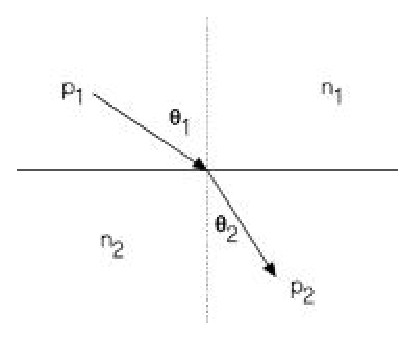
\includegraphics[width=200px, height=200px]{me20b020/ME20B020.eps}
\caption{Light changes its direction of propogation as it passes through an interface of two diffrent medium}
\label{fig:lightpropogation}
\end{figure}
Snell's Law serves as backbone for Optics and related studies, with every application of refractive optics relying on this formula. It can predict the movement of light thorugh surfaces (refer fig.(\ref{fig:lightpropogation})) and this has led to countless applications. It is used while making lens for spectacles and experimental purposes. 